\chapter{Desenvolvimento do projeto}
\label{chap:metod}

Nesta seção será descrito o procedimento utilizado para construção inicial do site portfólio do cliente, incluindo as fases conceitual e de design. Serão apresentados a ideação do projeto, os requisitos levantados, as tecnologias utilizadas, bem como a implementação e testes realizados ao longo do processo de desenvolvimento.

\subsection{Metodologia do projeto}
A metodologia utilizada para o desenvolvimento deste projeto foi uma abordagem híbrida, combinando elementos do modelo \textit{Waterfall} (cascata) com práticas do framework ágil \textit{Scrum}. Essa combinação permitiu maior controle nas fases iniciais e flexibilidade durante o desenvolvimento e validação com o cliente.

A estrutura do projeto seguiu a divisão em dois marcos principais de validação, denominados \textbf{Gate A} e \textbf{Gate B}, conforme descrito abaixo:

\begin{itemize}
    \item \textbf{Gate A – Planejamento e Levantamento:} Envolveu a coleta de informações com o cliente, definição dos requisitos funcionais e não funcionais, levantamento das preferências visuais, e alinhamento de expectativas com a equipe.
    
    \item \textbf{Gate B – Design e Validação Inicial:} Desenvolvimento dos primeiros esboços visuais e protótipos navegáveis. Criação de diagramas sobre o projeto. Apresentação ao cliente para validação e ajustes antes da implementação final.
\end{itemize}

A partir dessas etapas, o projeto foi estruturado com base nas seguintes fases:

\begin{itemize}
    \item \textbf{Levantamento de Requisitos:} Entendimento das necessidades do cliente por meio de reuniões e formulários, determinando preferências estéticas e funcionalidades desejadas.
    \item \textbf{Criação de Diagramas:} Elaboração de diagramas como o Diagrama de Casos de Uso, Diagrama de Classes e Diagrama de Atividades para representar visualmente os requisitos, funcionalidades e fluxos do sistema.
    \item \textbf{Design e Prototipação:} Criação de um layout visual com base no estilo minimalista, utilizando as cores preto e roxo, com foco em uma navegação de página única (scroll único).
    \item \textbf{Implementação:} Desenvolvimento do site utilizando as tecnologias HTML, CSS e JavaScript, com a hospedagem realizada por meio do GitHub Pages.
    \item \textbf{Entrega Final:} Finalização do projeto com a publicação do site, garantindo que todos os requisitos definidos foram atendidos.
\end{itemize}



\section{Ideação}

Nesta seção será apresentada a fase de ideação do projeto, que consistiu no processo inicial de concepção do site portfólio, alinhado às necessidades e preferências do cliente. Foram realizadas reuniões e o preenchimento de um formulário detalhado, com o objetivo de coletar informações essenciais para guiar o desenvolvimento.

Durante essa etapa, buscou-se compreender o perfil do cliente, seu estilo pessoal, suas áreas de interesse na área de tecnologia, bem como suas expectativas em relação ao design e às funcionalidades do site. Com base nesses dados, a equipe iniciou a definição dos objetivos do projeto, elaborou os primeiros esboços e estruturou a base para os requisitos e diagramas que orientaram as próximas fases do desenvolvimento.

A ideação permitiu garantir que o site refletisse a personalidade do cliente, adotando uma abordagem minimalista com um toque descontraído, incorporando cores específicas (preto e roxo), navegação em scroll único, e conteúdo organizado em formato de lista, como solicitado.


\subsection{Arquitetura da solução}

A arquitetura geral do projeto, representada na Figura \ref{fig:Arquitetura da solução}, ilustra de forma simplificada a estrutura do site portfólio desenvolvido, destacando a interação entre o usuário, as páginas do site e os recursos utilizados para hospedagem e funcionamento.

\begin{figure}[h!]
    \centering
    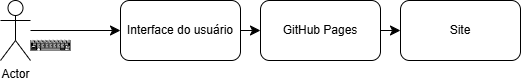
\includegraphics[width=0.8\textwidth]{solucao.drawio (1).png}
    \caption{Arquitetura da solução}
    \caption*{Fonte: Autoria própria.}
    \label{fig:Arquitetura da solução}
\end{figure}

A interface do usuário foi desenvolvida com tecnologias como HTML, CSS e JavaScript, proporcionando uma experiência visual responsiva, fluida e interativa. O site segue o modelo de página única (scroll único), em que todas as seções são acessadas verticalmente sem a necessidade de redirecionamentos.

O conteúdo do portfólio é exibido em seções organizadas, como “Sobre Mim”, “Estilo”, “Tecnologias” e “Certificados”. O sistema permite ainda a visualização de diplomas em formato de modal, além de conter redirecionamentos para redes sociais como GitHub e LinkedIn.

Para a hospedagem e disponibilização pública do projeto, foi utilizado o serviço do GitHub Pages, que permite o carregamento direto dos arquivos estáticos do repositório, garantindo fácil acesso ao site por meio de um link web. A arquitetura adotada garante simplicidade, manutenibilidade e acessibilidade para o cliente final.

\subsection{Requisitos Técnicos}

Nesta subseção, são apresentados os principais requisitos técnicos que nortearam o desenvolvimento do projeto, incluindo as ferramentas tecnológicas utilizadas, a organização da equipe e os métodos de acompanhamento do progresso.

\subsubsection{Ferramentas Tecnológicas}

O desenvolvimento do site foi realizado com base em tecnologias amplamente utilizadas no desenvolvimento web:

\begin{itemize}
\item \textbf{HTML5:} Utilizado para a estruturação semântica do conteúdo das páginas.
\item \textbf{CSS3:} Aplicado para a estilização e construção de um layout responsivo, garantindo boa experiência visual em diferentes dispositivos.
\item \textbf{GitHub Pages:} Plataforma utilizada para a hospedagem do site, possibilitando o acesso público ao projeto por meio de navegadores web.
\end{itemize}

\subsection{Modelagem dos processos}

A Figura \ref{fig:Modelagem dos processos} apresenta o fluxo de atividades realizadas durante o desenvolvimento do site portfólio, organizado em seis etapas sequenciais. O processo teve início com a coleta de informações junto ao cliente, na qual foram discutidas as necessidades, preferências estéticas e funcionalidades esperadas.

Na etapa seguinte, foi realizada a definição do layout e estilo visual, estabelecendo diretrizes como cores predominantes, tom da comunicação e escolha de ícones, com base nas preferências levantadas. Em seguida, procedeu-se com a estruturação do conteúdo, organizando as seções do portfólio e os textos informativos a serem exibidos.

Com o conteúdo e estilo definidos, passou-se à codificação do site em HTML e CSS, aplicando os conhecimentos técnicos para transformar o design em uma interface funcional. Após isso, foi feita a publicação do site na plataforma GitHub Pages, tornando-o acessível pela web.

Por fim, realizou-se a etapa de testes, ajustes e coleta de feedback, na qual o site foi avaliado para garantir a conformidade com os requisitos estabelecidos e permitir eventuais melhorias com base no retorno do cliente.

\begin{figure}[h!]
    \centering
    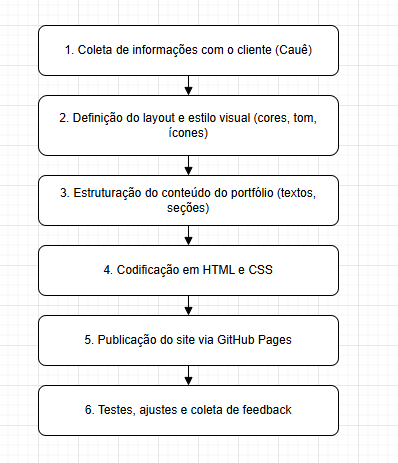
\includegraphics[width=0.8\textwidth]{fluxo_processos_desenvolvimento.png}
    \caption{Modelagem dos processos}
    \caption*{Fonte: Autoria própria.}
    \label{fig:Modelagem dos processos}
\end{figure}